\chapter{Example}
	% A little explanation beforehand
    This chapter will show how to develop a simple example by installing \Kieker\ before marking some code lines for the monitoring. After the necessary data has been collected, they will be analyzed by an own developed component. The example itself is available on the website of \Kieker.
	
	\section{Download and Installation}
      \Kieker\ can be downloaded from \KiekerDownloadUrl. The content of the zip- respectively the tar.gz-file should be extracted to any directory, which we will call ``\KiekerDir`` within this tutorial. The installation of \Kieker\ is completed.\\
      If desired, the new created path can of course be assigned to an easy remindable environment variable. 
 
    \section{Monitoring}
      For the creation of the example it is recommended to create a new working directory (e.g. ''example'') of the following structure:
      \begin{center}
		  \dirtree{%
		  .1 example\DTcomment{The root directory of the project}.
		  .2 build\DTcomment{The directory for the compiled class files for Java}.
		  .2 lib\DTcomment{The directory for the libraries and needed jar-files}.
		  .3 \monitoringCtrlJar\DTcomment{}.
		  .3 \commonJar\DTcomment{}.
		  .3 commons-logging-1.1.1.jar\DTcomment{}.
		  .2 src\DTcomment{The directory for the sourcecode files}.
		  .3 mySimpleKiekerExampleManual\DTcomment{The directory for the new package}.
		  .4 CRM.java\DTcomment{One of the sourcecode files}.
		  .4 Catalog.java\DTcomment{One of the sourcecode files}.
		  .4 Bookstore.java\DTcomment{One of the sourcecode files}.
		  .4 BookstoreStarter.java\DTcomment{One of the sourcecode files}.
		  }      
      \end{center}
	  The listed jar-files must be copied from the \Kieker\ directory:
      \begin{itemize}
		\item \KiekerDir/dist/\commonJar\
		\item \KiekerDir/dist/\monitoringCtrlJar\
		\item \KiekerDir/lib/commons-logging-1.1.1.jar
      \end{itemize}
      The sourcecode files consist of the following lines:
      % It isn't necessary to do this every time but it makes sure that the listing has the correct format.
      \setJavaCodeListing

	  % If the Path to the examples changes, then they have to be changed here AS WELL!!
      \lstinputlisting[caption=Bookstore.java]{source-example/manual-monitoring/src/mySimpleKiekerExampleManual/Bookstore.java}

	  % Due to this package we have to write the important part manually...
	  \begin{lstlisting}[caption=BookstoreStarter.java]
		package mySimpleKiekerExampleManual;

		import kieker.analysis.plugin.MonitoringRecordConsumerException;
		import kieker.analysis.reader.MonitoringLogReaderException;

		public class BookstoreStarter {
			public static void main(String[] args) throws MonitoringLogReaderException,
				MonitoringRecordConsumerException {
				/* Start the monitoring */
				Bookstore.startBookstoreRequests();
			}

		}
	  \end{lstlisting}
	  
      \lstinputlisting[caption=CRM.java]{source-example/manual-monitoring/src/mySimpleKiekerExampleManual/CRM.java}

      \lstinputlisting[caption=Catalog.java]{source-example/manual-monitoring/src/mySimpleKiekerExampleManual/Catalog.java}
	  
      The monitoring itself is done manually. Although this is not the strength of \Kieker\ it is pretty good for a quick start.
	  
      % Make sure that this listing will be modified, once the sourcecode changes!!! 
	  % It must show the whole monitoring of the bookstorecall, from getting the first time to persisting of the record!!
      \lstinputlisting[firstline=20, lastline=29, caption=Cutting from Bookstore.java, label=listing:cuttingBookstore]{source-example/manual-monitoring/src/mySimpleKiekerExampleManual/Bookstore.java}
	  
      In Listing \ref{listing:cuttingBookstore} can be seen, how the monitoring itself is done. We remember the time before and after a specific method call (in this case: \textit{searchBook()}). These informations are stored in the so called operation execution record. Its (partially) layout can be seen in Figure \ref{image:operationexecutionrecordclassdiagram}.
	  
	  % This figure contains the short class diagram of the operation execution record.
		\begin{figure}[H]
			\begin{center}
				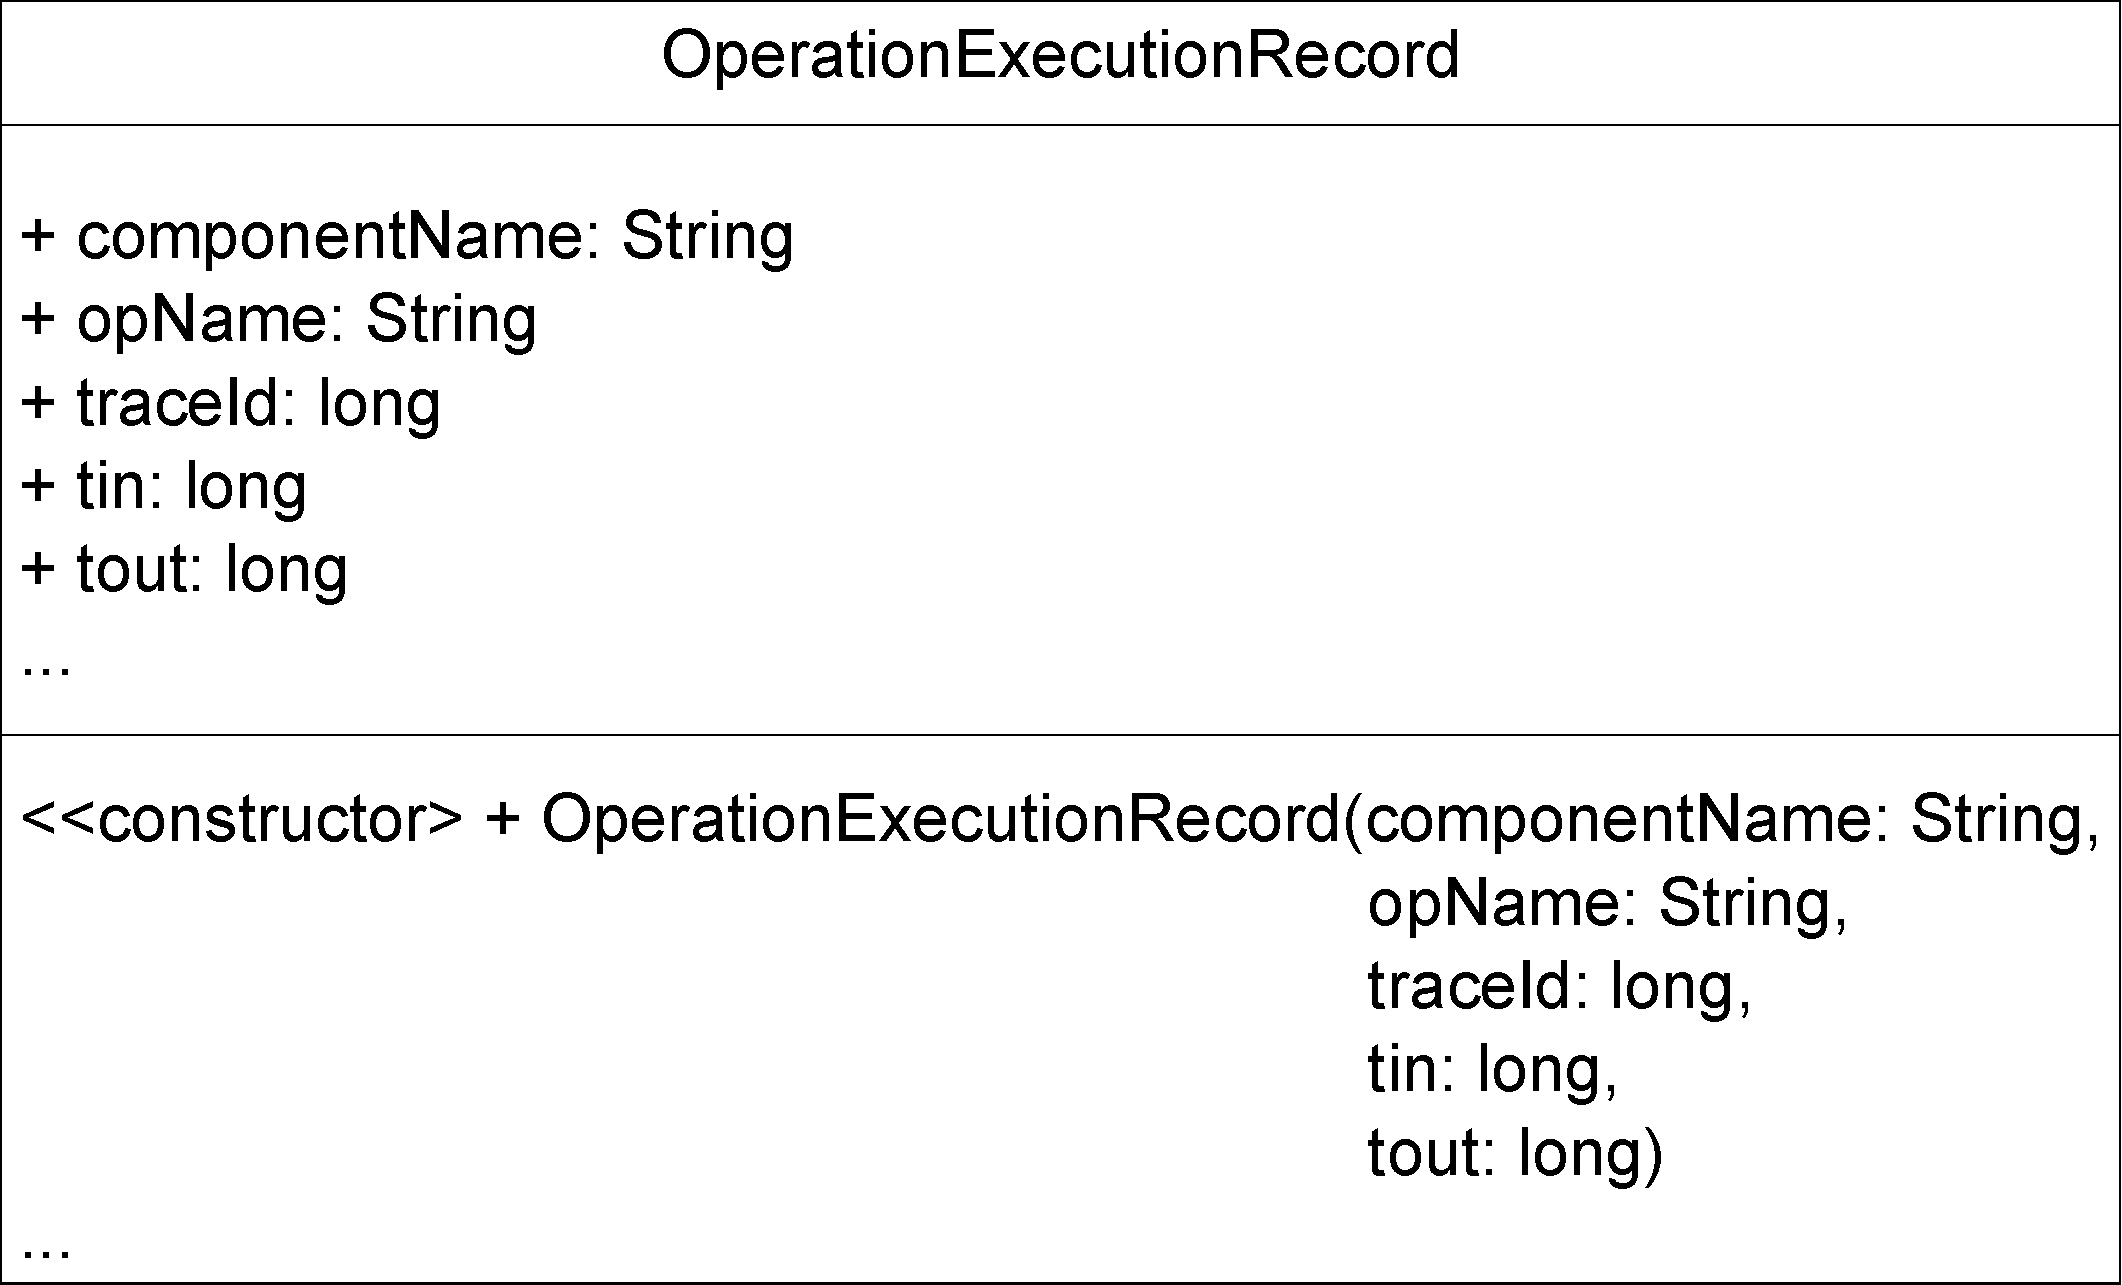
\includegraphics[width=0.4\textwidth]{./images/OpExRecClassDiagram.pdf}
				\caption{The class diagram of the operation execution record}
				\label{image:operationexecutionrecordclassdiagram}
			\end{center}
		\end{figure}
	  
		The important attributes are:
		\begin{itemize}
			\item The component (the class) in which the called method is.
			\item The called method.
			\item The trace id of the current trace we want to record. Due to the fact, that we follow only one trace, this is zero in all recordings.
			\item The time before the sourcecode which should be measured.
			\item The time after the sourcecode which should be measured.
		\end{itemize}
		  
		The sourcecode should now be compilable and executable:
		
		% We need something like the ouput from the bash.
		
		\setBashListing
		% Note: This is different under Windows and Linux!!
		% If the Kieker-Dir for the tutorial is changed, make sure that this is done here as well!!
		% We cannot put a latex-macro within the listing!
		\begin{lstlisting}
			nils@Laptop:~/example$ javac src/mySimpleKiekerExampleManual/*.java\
			-classpath\
			./lib/kieker-common-1.5-trunk.jar:\
			./lib/kieker-monitoring-1.5-trunk.jar:\
			-d build

			nils@Laptop:~/example$ java -Dlog4j.configuration=$<$KIEKER-DIR$>$/META-INF/log4j.properties\
			-classpath\
			./build/:\
			./lib/kieker-common-1.5-trunk.jar:\
			./lib/kieker-monitoring-1.5-trunk.jar:\
			./lib/commons-logging-1.1.1.jar\
			mySimpleKiekerExampleManual.BookstoreStarter
		\end{lstlisting}
		If the sourcecode should be compiled and executed under Windows, the paths have do be sepereated with semicolons instead of colons. Furthermore it is not possible to wrap the single parts of the commands with a backslash.\\
		If everything worked correctly, there should now be a new directory named ``tpmon-20100605-115948636-UTC'' (just with other numbers) in the default temporary directory (under Linux this should be ``/tmp''; under Windows ``C:/temp''). In this directory, there should be a file with the extension ``.dat'' which contains the recorded informations from the source code. A possible content of this file can be found in the appendix of this tutorial.\\
		Now we take a closer look at the analysis.

	\section{Analysis}
      % Here we go...we have to inform the user of the programs he need for the converting. And that means as well, that a window user cannot do this part.
      For the visualization via \Kieker\ we need the both tools graphviz (\url{www.graphviz.org/}) and plotutils (\url{www.gnu.org/software/plotutils/}).\\
      Assume that we already have our recorded informations saved in a ``.dat''-file somewhere for example in the ``tmp``-directory, we can now start with converting these informations into graphs. For the first, we change into our \Kieker\-directory ($\sim$/kieker). It is recommended to create a new directory for the graphs first:
      \begin{lstlisting}
	nils@Laptop:~/kieker$ mkdir /tmp/graphs
      \end{lstlisting}
      The shell-script ''./bin/trace-analysis.sh`` will now do most of the job. It starts the analysis and uses the above-mentioned tools to convert to files into graphs and diagrams.
      \begin{lstlisting}
	nils@Laptop:~/kieker$ ./bin/trace-analysis.sh --plot-Sequence-Diagrams --short-labels -i /tmp/tpmon-20100606-112536844-UTC/ -o /tmp/graphs/
      \end{lstlisting}
	The command ''--plot-Sequence-Diagrams`` tells the shell script to convert our data into a sequence diagram\footnote{Other diagrams and graphs can be plot of course as well. Start trace-analysis.sh without any parameters to see the possible commands.}; with ''--short-labels`` we make sure that the components get a shorter name and the directories after ''-i`` and ''-o`` are the input- and the output-directories. If everything went well, \Kieker\ converted the data into files, which can now converted directly into visual graphs:
	\begin{lstlisting}
	  nils@Laptop:~/kieker$ ./bin/dotPic-fileConverter.sh /tmp/graphs/ svg
	\end{lstlisting}
	The shell script ''./bin/dotPic-fileConverter.sh`` gets the directory with the files and the desired file extension (e.g. svg or png). The resulting graphs should now be available in ''/tmp/graphs`` and should look like figure \ref{image:sequencediagram}
	% This is the simple sequence diagram which results by running the bookstore example; of course without showing the traces etc.
	\begin{figure}[H]
	  \begin{center}
	    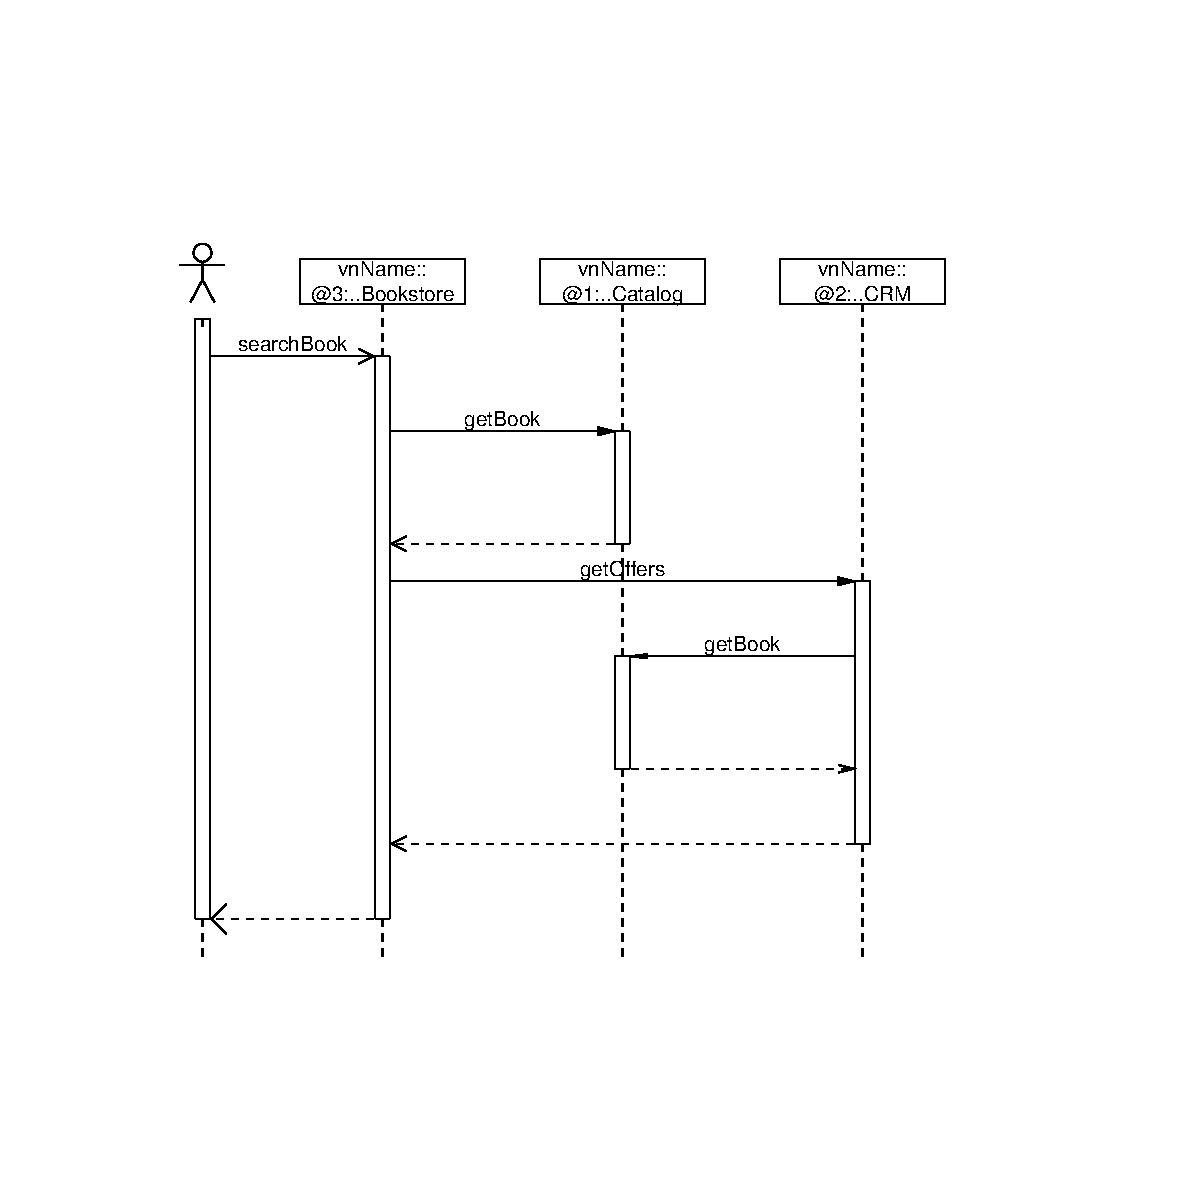
\includegraphics[width=0.7\textwidth]{sequenceDiagram.pdf}
            \caption{The resulting sequence diagram}
	    \label{image:sequencediagram}
	  \end{center}
	\end{figure}
	We are now able to monitor source code and to visualize these recorded informations in a simple way.

    \section{Using AOP}
      Now we want to monitor whole methods without surrounding the method calls with a block where we keep the time manually. We will now use so called annotations to mark the methods we want to monitor\footnote{To be more precisely: We use annotations which will then be used by the aspect-oriented Java extension named AspectJ to surround the method calls with code blocks which are similar to these, we already used manually.}. As can be seen in the following listing we write the annotation \textit{kieker.monitoring.annotation.TpmonExecutionMonitoringProbe} above the methods to be monitored. 
      \setJavaCodeListing
      \lstset{caption=Bookstore.java, label=listing:Bookstore2.java}
      \lstinputlisting{source-example/annotation-monitoring/src/mySimpleKiekerExample/bookstoreTracing/Bookstore.java}
      Due to the use of AspectJ we need now to copy the file ''META-INF/aop.xml.example`` from our \Kieker\ directory to our working directory to ''META-INF/aop.xml``. This file tells AspectJ which parts of our source code should be monitored. To inform AspectJ about our own annotations, we need another libarary as well. We copy $\sim$/kieker/dist/kieker-tpmon-\version\_ctw.jar to our own example project in $\sim$/example/lib/kieker-tpmon-\version\_ctw.jar\\
      To make sure that every method in our program which is annotated will be monitored, we have to write the following into the ''aop.xml``:
      \setXMLListing 
      \begin{lstlisting}
	<aspectj>
	  <!-- turn verbose on to check which files are instrumented -->
	  <!-- <weaver options="-verbose"/> -->
	  <weaver options="">
	      
	  <!-- The following line is the important one -->
	  <include within="*"/> 

	  <!-- uncomment following to instrument sun jpetstore -->
      \end{lstlisting}
      The compiling is pretty much the same as before (except for some more libraries), but in order to run the program, we have to copy the configuration files into the build-directory.
      % Same as before. If the libraries change, this has to be modified as well.
      \begin{lstlisting}
	nils@Laptop:~/example$ javac ./src/mySimpleKiekerExample/bookstoreTracing/Bookstore.java ./src/mySimpleKiekerExample/bookstoreTracing/Catalog.java ./src/mySimpleKiekerExample/bookstoreTracing/CRM.java -classpath ./lib/kieker-monitoring-1.5-trunk_ctrl.jar:./lib/commons-logging-1.1.1.jar -d build/
	nils@Laptop:~/example$ cp -r ./META-INF/ ./build/META-INF
	nils@Laptop:~/example$ java -Dlog4j.configuration=META-INF/log4j.properties -javaagent:lib/aspectjweaver-1.6.6.jar -Dorg.aspectj.weaver.showWeaveInfo=true -Daj.weaving.verbose=true -classpath ./build/:./lib/kieker-monitoring-1.5-trunk_ctrl.jar:./lib/commons-logging-1.1.1.jar:./lib/kieker-monitoring-1.5-trunk_ctw.jar mySimpleKiekerExample.bookstoreTracing.Bookstore
      \end{lstlisting}